\chapter{Introduzione}
In questo capitolo presenterò gli aspetti matematici fondamentali per andare ad affrontare gli argomenti del corso.
\\
\section{Vettori e matrici}
Denotiamo un vettore riga e colonna rispettivamente con $(a,b,c)$ e $ \begin{bmatrix} a \\ b \\ c \end{bmatrix} $
\\dove $a,b,c\in\mathbb{R}$ sono scalari.
\\
In generale denotiamo con le lettere maiuscole le matrici, e.g. $X$ e i suoi elementi con $X_{ij}$.\\
$x\in \mathbb{R}^n$ è un vettore di n elementi e $X \in \mathbb{R}^{m \times n}$ è una matrice di dimensione $m \times n$.
\section{Norme di vettori e matrici}
Dato un vettore $x\in \mathbb{R}^n$ vi sono diversi tipi di norme comunemente utilizzate.
\begin{itemize}
	\item $||x||_2=(\sum_{i=1}^n x_i^2)^{\frac{1}{2}}$
	è il tipo più comune e viene chiamato \textbf{norma 2} di un vettore o \textbf{norma Euclidea}. Normalmente è denotato semplicemente con $||x||$.
	\item $||x||_1=|x_1|+|x_2|+\cdots+|x_n|$, detta la \textbf{norma 1} o \textbf{distanza di Manhattan}
	\item $||x||_\infty=\max_{1\leq i\leq n}|x_i|$, detta la \textbf{norma $\infty$}.
\end{itemize}
Analogamente, per una matrice $X \in \mathbb{R}^{m \times n}$, si possono definire diverse norme:

\begin{itemize}
	\item \textbf{Norma di Frobenius}: $||X||_F = \left( \sum_{i=1}^m \sum_{j=1}^n |X_{ij}|^2 \right)^{\frac{1}{2}}$
	\item \textbf{Norma spettrale (o norma 2)}: $||X||_2$
	\item \textbf{Norma 1}: $||X||_1=\sum_{i,j} |X_{ij}|$
\end{itemize}
\section{Notazioni generiche}
Siano:
\begin{itemize}
	\item $u$: variabile indipendente (input), non necessariamente un vettore o uno scalare
	\item $v$: variabile dipendente (output), come sopra 
\end{itemize}
allora abbiamo che:
\begin{itemize}
	\item $x=\phi(u)$, dove $x\in \mathbb{R}^d$ è il vettore di features e $\phi$ è la funzione di mapping o embedding.
	\item $y=\psi(v)$, dove $y\in \mathbb{R}^m$ è il vettore target (o di output) e $\psi$ è la funzione di mapping di feature in output.
\end{itemize}
Siano $x^1,\dots x^n$ e $y^1,\dots y^n$ due dataset di $n$ esempi, dove $x^i$ e $y^i$ formano la $i$-esima coppia di dati. Dunque $n$ è il numero di campioni, allora posso associarvi le due matrici dei dati
$$X=\begin{bmatrix}
	(x^1)^T\\ \vdots \\ (x^n)^T
\end{bmatrix}\in \mathbb{R}^{n \times d}, \quad Y=\begin{bmatrix}
	(y^1)^T\\ \vdots \\ (y^n)^T
\end{bmatrix}\in \mathbb{R}^{n \times m}$$
Le cui righe sono i vettori feature e i vettori target rispettivamente, trasposti.\\
Definiamo allora:
\begin{itemize}
	\item $g_\theta: \mathbb{R}^d \to \mathbb{R}^m$ è un predittore. 
	\item $\hat{y}=g_\theta(x)$ è la predizione di $y$, dato $x$.
	\item $\theta\in\mathbb{R}^p$ è il vettore di parametri del predittore.
\end{itemize}
La scelta dei parametri $\theta$ a seconda dei dati viene chiamato \textit{training} o \textit{fitting} del predittore. 
\\
Separando le definizioni in base al dominio di riferimento, abbiamo le seguenti suddivisioni:
\begin{itemize}
	\item Spazio di input:
	\begin{itemize}
		\item Istanza (sample, oggetto, record): un esempio descritto da un certo numero di attributi.
		\item Attributo (campo, caratteristica, variabile): misura di un aspetto di una istanza.
	
	\end{itemize}
	\item Spazio di output:
	\begin{itemize}
		\item Classe (label, target): categoria a cui appartiene una istanza.
	\end{itemize}
	\item Predittore o modello:
	\begin{itemize}
		\item Una funzione $g$ con parametri $\theta$ che dato uno spazio di input $X$ produce uno spazio di output $Y$.produce una predizione nello spazio di output $Y$.
	\end{itemize}
\end{itemize}

\begin{figure}[H]
	\centering
	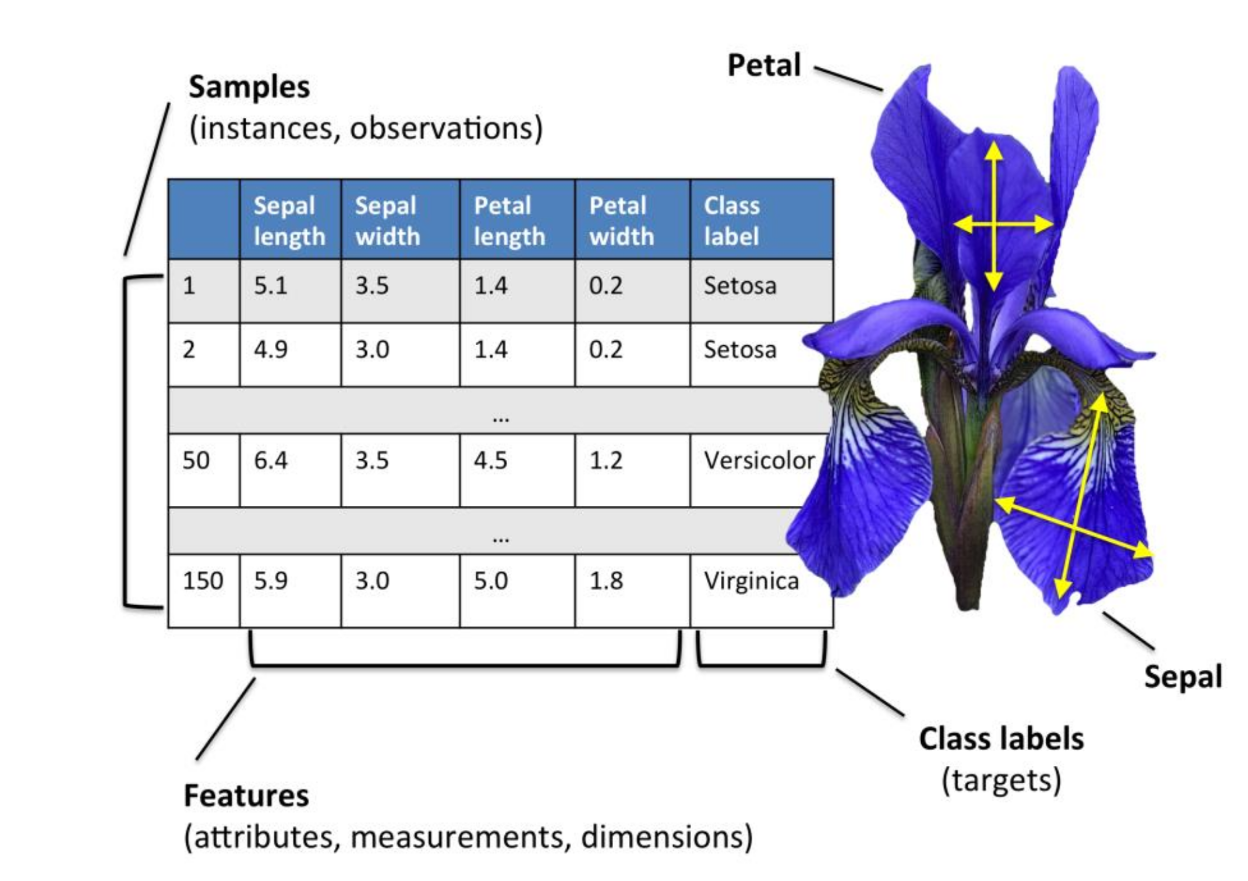
\includegraphics[width=0.6\textwidth]{pictures/esempioDefinizioni.png}
	\caption{Esempi pratici.}
\end{figure}
\begin{figure}[H]
	\centering
	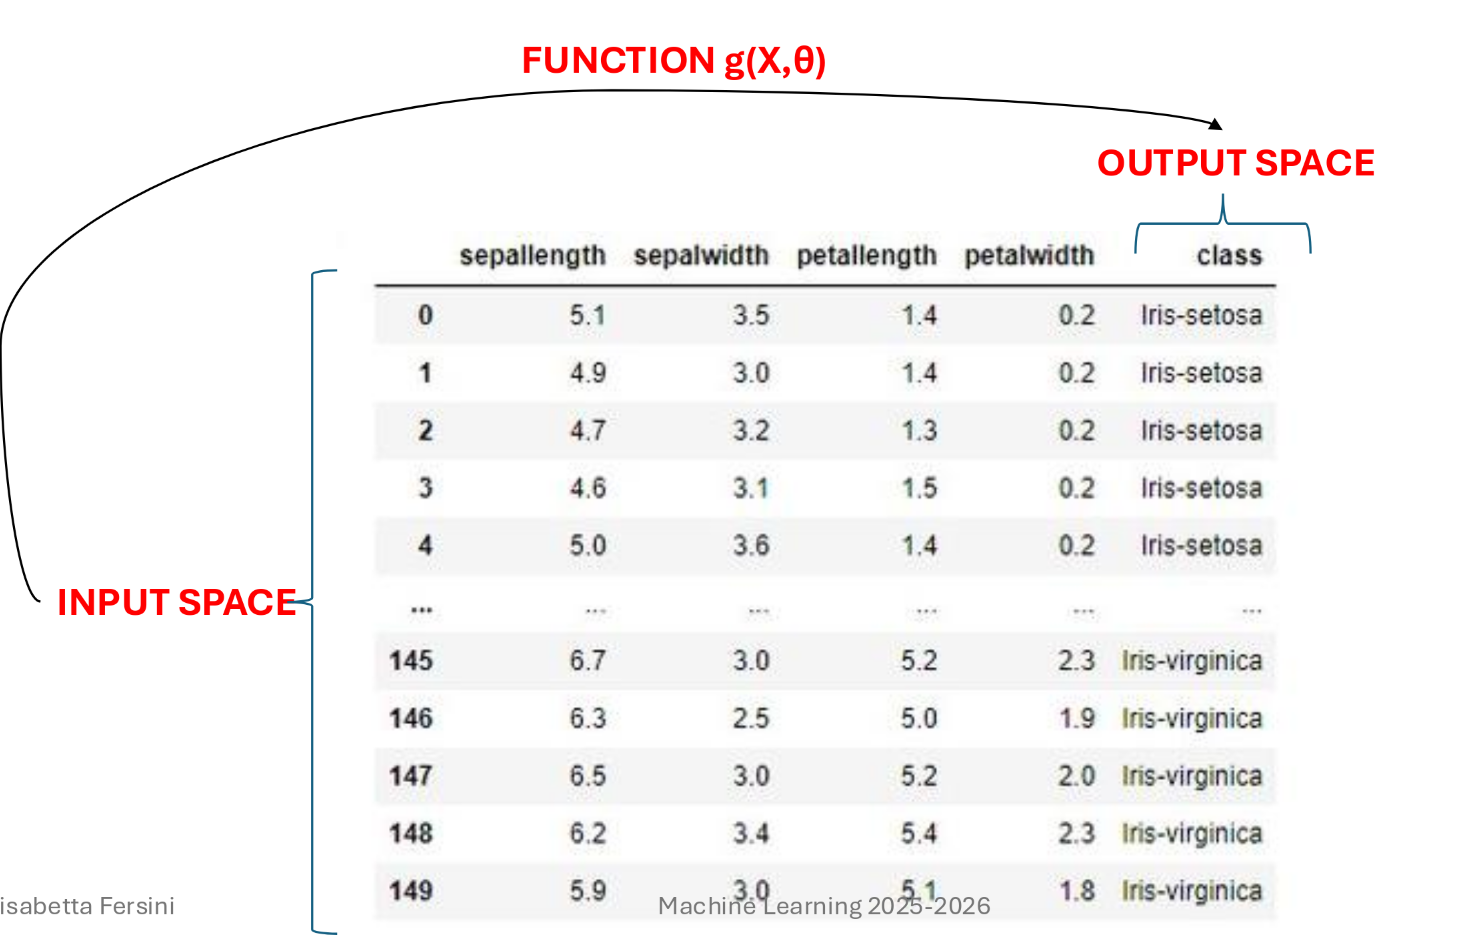
\includegraphics[width=0.6\textwidth]{pictures/esempioDefinizioni2.png}
	\caption{Esempi pratici 2.}
\end{figure}
\begin{figure}[H]
	\centering
	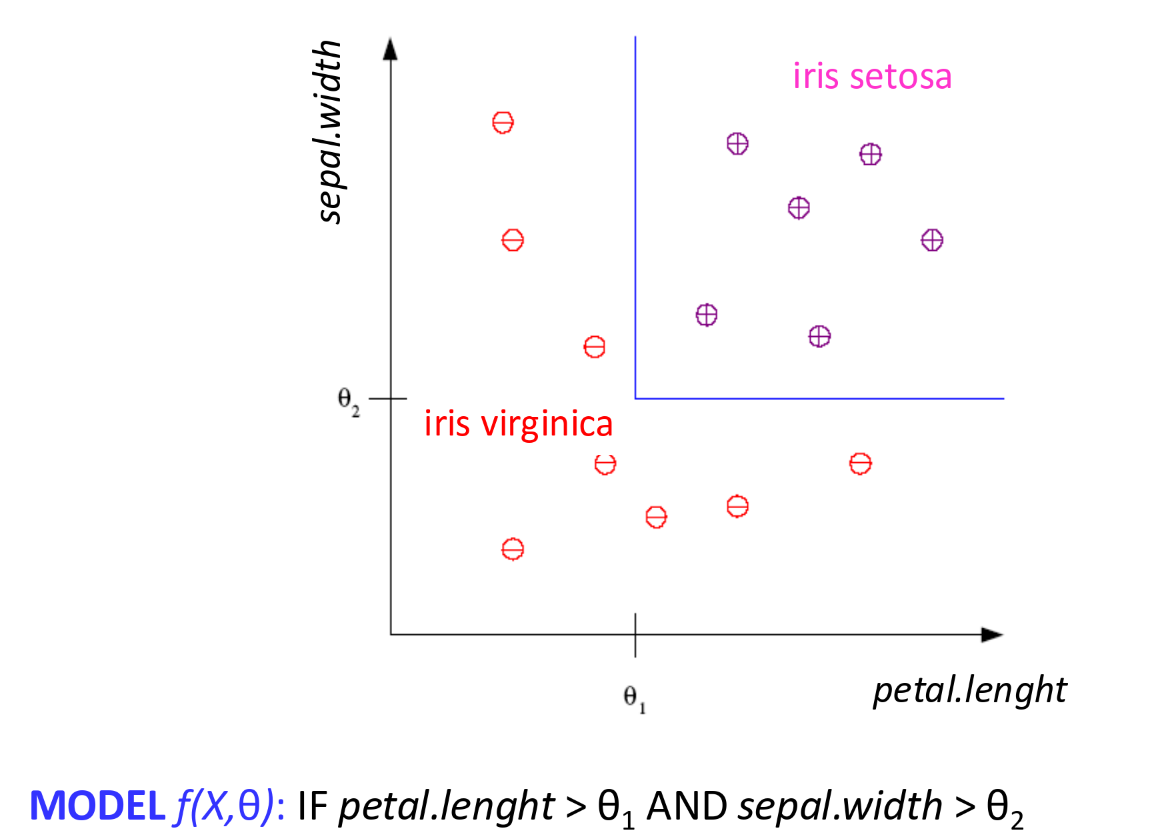
\includegraphics[width=0.6\textwidth]{pictures/esempioDefinizioni3.png}
	\caption{Esempi pratici 3.}
\end{figure}
\section{Rischio atteso e rischio empirico}
Quando un modello di machine learning $g$ viene addestrato, vogliamo che abbia buone prestazioni non solo per i dati utilizzati per il training, ma anche per dati sconosciuti (\textit{generalizzazione}).
Dovremo stimare il \textbf{rischio atteso}, ovvero la loss media che dovrebbe presentarsi sulla reale distribuzione dei dati $P(x,y)$. 
\\
Supponiamo di avere un dataset di $n$ coppie $(x^i,y^i)$, dove $x^i$ è il vettore di feature e $y^i$ il vettore target associato alla $i$-esima istanza.
Definiamo la \textbf{loss function} $L(g_\theta(x),y)$, che misura l'errore commesso dal modello $g_\theta$.
\\
Dunque il rischio atteso è definito come:
$$R(g_\theta)=E_{(x,y)\sim P}[L(g_\theta(x),y)]$$
Da notare però che la reale distribuzione $P$ \underbar{non è nota}, dunque non possiamo stimare il rischio atteso. Le cause sono:
\begin{enumerate}
	\item Distribuzione non nota \\
		Osserviamo solo un campione finito di campioni estratti dal mondo reale. La distribuzione completa che genera quei dati non è accessibile.
	\item Impossibilità pratica\\
		Anche se conoscessimo il processo di generazione in teoria, calcolare esattamente la predizione del rischio è impossibile in generale perché richiederebbe di sommare/integrare tutte i possibili esempi.
	\item Dati finiti e rumorosi\\
		Il dataset a disposizione è finito, spesso presenta rumore e errori di misura, o bias di raccolta. Dunque possiamo solo approssimare il rischio utilizzando una \textbf{stima empirica}.
\end{enumerate}
Dunque, vogliamo stimare e minimizzare il rischio empirico. Supponiamo di avere un dataset di $n$ coppie $(x^i,y^i)$.
Definiamo la loss function $L(g_\theta(x),y)$, che misura l'errore commesso dal modello $g_\theta$.
Allora il rischio empirico $\hat{R}(g_\theta)$ è definito come:
$$\hat{R}(g_\theta)=\frac{1}{n}\sum_{i=1}^n L(g_\theta(x^i),y^i)$$
La maggior parte degli algoritmi di machine learning minimizzano il rischio empirico.
$$g^*=arg\min_{g_\theta\in G}\hat{R}(g_\theta)$$
Dunque dato un dataset di training, $x_i,y_i$ per $i=1,\dots n$, per cui la loss sull' $i$-esima coppia di dati è $l(g_\theta(x_i),y_i)$, il rischio empirico è la loss media sul dataset di training.
L'empirical risk minimization (ERM) si occupa di scegliere i parametri $\theta$ che minimizzano il rischio empirico.
\section{Estrazione delle features}
Utilizziamo $u$ per denotare i dati di input grezzi, ad esempio un vettore, testo, immagine, audio, video, ecc.
$x=\phi(u)$ è il vettore di features, ottenuto tramite la funzione $\phi$, chiamata embedding, funzione feature o mappamento di feature. La funzione $\phi$ può variare molto nel livello di complessità in base al caso.
\section{Modelli}
Noi cerchiamo un predittore (o modello) $g_\theta:\mathbb{R}^d\to \mathbb{R}^m$ che dato un vettore di features $x\in \mathbb{R}^d$ produce una predizione $\hat{y}=g_\theta(x)\in \mathbb{R}^m$.
La scelta del modello $g_\theta$ viene effettuata sia in basa ai dati a disposizione che in base alle conoscenze pregresse.
In termini di dati grezzi, il predittore è  $\hat{v}=\psi^{-1}(g(\phi(u)))$, con qualche variante se la funzione $\psi$ è invertibile.
Se $\hat{y}\approx y$ allora il predittore ha fatto una buona predizione sulla $i$-esima coppia di dati. Però, l'obiettivo è avere $\hat{y}\approx y$ non solo sui dati di training, ma anche su dati mai visti prima.
Due forme equivalenti per rappresentare un modello sono $\hat{y}=g_\theta(x)$ e $\hat{y}=g(x,\theta)$. Si dice che la funzione $g$ da la struttura (o forma) del predittore, $\theta$ è un parametro per il modello predittivo
La scelta di un particolare $\theta\in \mathbb{R}^p$ si chiama \textit{tuning} o \textit{fitting} o \textit{addestramento} del modello.
Un algoritmo di apprendimento è una ricetta per scegliere i parametri $\theta$ a partire dai dati di training.
\section{Assunzione $i.i.d.$}
Prima di presentare il concept learning è necessario presentare l'assunzione $i.i.d.$ (independent and identically distributed).
Dunque si assume che i dati siano stati campionati in modo indipendente e che provengano dalla stessa distribuzione.
\begin{itemize}
		\item 
		In teoria : L'unione delle funzioni di distribuzione di probabilità possono essere scritte come il prodotto delle funzioni di distribuzione di probabilità marginali.
		\[
		f(X,\theta)=\prod_{i=1}^n f(X_i,\theta)
		\]
	\item 
		In pratica: Ogni modello considera un campione alla volta, ignorando le feature degli altri campioni.
\end{itemize}
\begin{figure}[h]
	\centering
	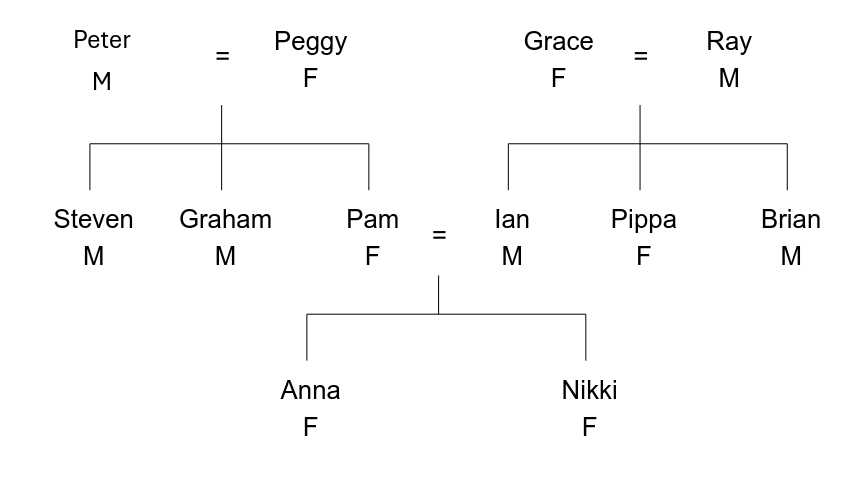
\includegraphics[width=0.5\textwidth]{pictures/familyTree.png}
	\caption{Esempio di struttura familiare}
	\label{fig:iid}
\end{figure}
\begin{figure}
	\centering
	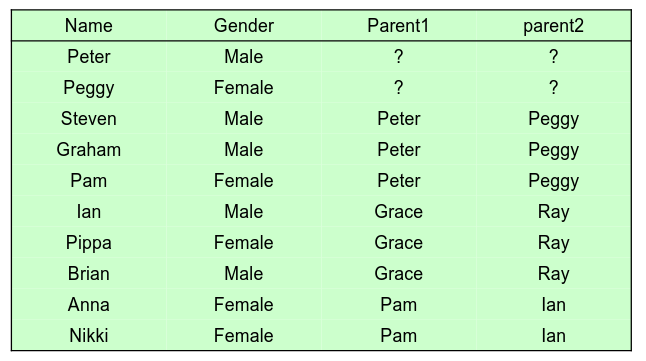
\includegraphics[width=0.5\textwidth]{pictures/familyTable.png}
	\caption{formato tabellare dei dati della figura \ref{fig:iid}}
	\label{fig:iid2}
\end{figure}
Possiamo notare che nella figura \ref{fig:iid2} sono presenti dei campi nulli, questo è dovuto al fatto che non tutti i dati sono stati raccolti, ciò presenta un problema.
Anche una rappresentazione relazionale dei dati può essere effettuata, come ad esempio in figura \ref{fig:iid3}.
\begin{figure}
	\centering
	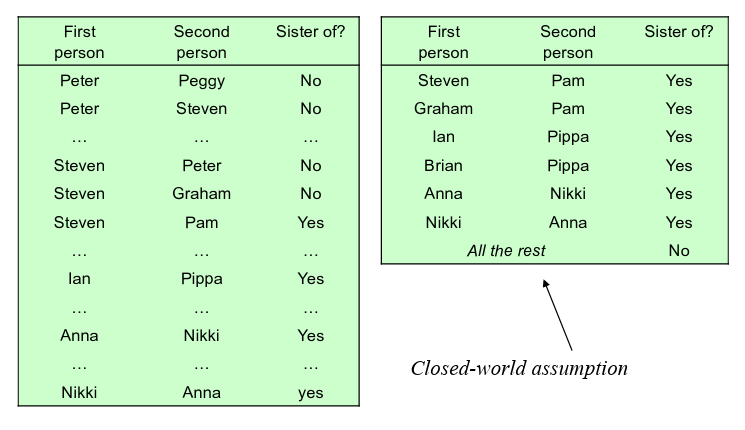
\includegraphics[width=0.6\textwidth]{pictures/familyRel.png}
	\caption{formato relazionale dei dati della figura \ref{fig:iid}}
	\label{fig:iid3}
\end{figure}
Infine è anche possibile combinare le due rappresentazioni, come in figura \ref{fig:iid4}.
\begin{figure}
	\centering
	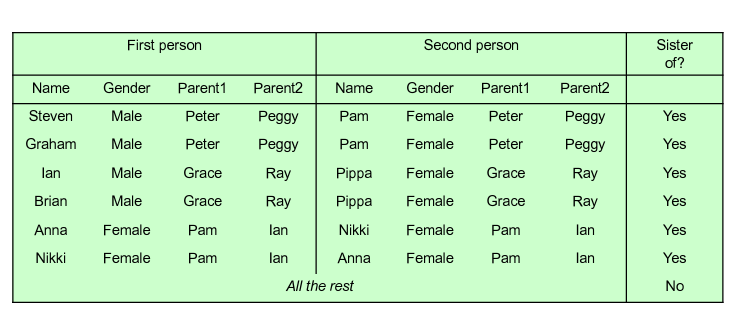
\includegraphics[width=0.6\textwidth]{pictures/familyComb.png}
	\caption{formato misto dei dati della figura \ref{fig:iid}}
	\label{fig:iid4}
\end{figure}\\
Il processo di \textbf{flattening} su un file è detto \textbf{proposizionalizzazione}, ovvero l'unione di più relazioni in una sola.
Questa operazione è possibile per ogni insieme finito di relazioni finite, Un problema che emerge è la presenza di relazioni senza un numero pre specificato di oggetti.
La proposizionalizzazione può introdurre delle regolarità fittizie che riflettono la struttura del database, inoltre possono introdurre dei \textbf{bias} causati da dati ripetuti.
\begin{figure}[H]
	\centering
	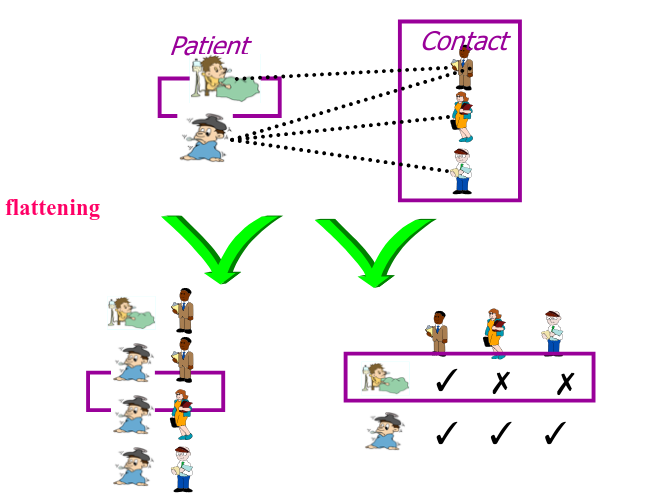
\includegraphics[width=0.5\textwidth]{pictures/flattening.png}
	\caption{esempio di flattening}
	\label{fig:flattening}
\end{figure}
\noindent
Nella colonna a sinistra della figura \ref{fig:flattening} possiamo notare che viene introdotto un bias dato dalla ripetizione di un dato, che in realtà è causato dalla natura relazionale dello stesso (dunque perdo la i.i.d.).
Mentre colonna di destra viene introdotto un bias dato che viene considerato come non avvenuto un evento che in realtà potrebbe essere ancora non stato osservato, inoltre assumo a prescindere il numero di attributi e questo causa problemi nel momento in cui ne vengono aggiunti di nuovi.
\section{tipi di attributi}
Ogni istanza è descritta da un numero fisso predefinito di feature, i suoi attributi.
Ci sono diversi tipi di attributi:
\begin{itemize}
	\item \textbf{Quantità nominali}:Valori a simboli distinti, i valori in sé servono solo come etichette o nomi.
		Non vi è nessuna relazione implicita tra i valori nominali, come ordine o distanza. L'unico test effettuabile è quello di eguaglianza.
	\item \textbf{Quantità ordinali}: Valori che possono essere ordinati, ma non vi è alcuna informazione sulla distanza tra i valori (addizione e sottrazione non hanno significato).
	\item \textbf{Quantità di ratio}: Il metodo di misurazione definisce lo zero, ad esempio una distanza. Assumono valori in $\mathbb{R}$ e sono dotati di un ordine naturale. Sono possibili tutte le operazioni aritmetiche.
\end{itemize}
Perché è importante conoscere il tipo di attributo? Operazioni e confronti tra attributi di tipi diversi potrebbero non avere senso al livello semantico. Inoltre ci permettono di effettuare un check sulla validità dei valori, gestire la mancanza di essi ed effettuare confronti di eguaglianza.
